%!TEX root = ../template.tex
%%%%%%%%%%%%%%%%%%%%%%%%%%%%%%%%%%%%%%%%%%%%%%%%%%%%%%%%%%%%%%%%%%%
%% chapter1.tex
%% NOVA thesis document file
%%
%% Chapter with introduciton
%%%%%%%%%%%%%%%%%%%%%%%%%%%%%%%%%%%%%%%%%%%%%%%%%%%%%%%%%%%%%%%%%%%
\newcommand{\novathesis}{\emph{novathesis}}
\newcommand{\novathesisclass}{\texttt{novathesis.cls}}

\chapter{Introduction}

Proteins are large molecules with complex structures which carry out a wide range of functions in organisms. They are essential to life due to their versatility since they can act as antibodies, to help combat viruses and bacteria, they can take the enzymatic role in order to increase the rate of chemical reactions in the body, they can aid in hormone creation, in the transport of small molecules, etc.

There are a few factors which determine the function of a given protein, namely its amino acid sequence and spatial conformation. Despite this, it is known that as time passes sequences undergo mutations to its amino acids. As such, if enough time goes by, a given sequence may become unrecognizable when comparing to what it used to be. Luckily, structures are not affected as heavily as sequences, which means that they tend to be much more conserved during a protein's evolution to the extent that they are a better tool for understanding their functionality, interactions and relationships.

In applications such as the ones mentioned ahead \cite{kufareva2011methods}, the value of protein structures is recognized and used to obtain insightful information:

\begin{itemize}

\item \textbf{Evolutionary analysis}

It is possible to identify common ancestors using both sequence and structural comparisons. If the proteins to compare have a relatively short evolutionary distance between each other, usually it is enough to compare the amino acid chains of both proteins to establish ancestry. The chains should be similar due to the short amount of time that has passed, which means the amino acid sequence shouldn't be significantly altered. However, this method works under the assumption that the changes to the sequences are minimal, which most likely will not happen if the evolutionary distances are greater. In this case, the most appropriate method is comparing the proteins by their three-dimensional structure which is better preserved than sequence. This approach may identify similarities among proteins because even if the amino acid sequence is changed as time passes, there will still be some elements with a layout similar to a previous state of the protein. In practice however, most cases are more complicated and thus, require more complex approaches which use combinations of both types of comparisons \cite{burkowski2008structural} \cite{holm1996mapping}. 

\item \textbf{Docking}

Another application where it is necessary to group and compare structures is protein docking \cite{halperin2002principles}. This is an expression that is used to describe computational methods that output predictions on how two proteins - a receptor and a ligand - interact in order to form a molecular complex. The details of these processes are beyond the scope of this work, but in short, protein docking is comprised of two stages: search and scoring. The first stage is where we search through every spatial arrangement of both molecules so we can obtain a set of those that might resemble the true conformation of the complex. The scoring stage is where the generated set is analyzed and ranked according to some function. Generated predictions can also compared to measure their quality. Since both the predicted and target complexes possess the same sequences, their sequence alignments are easy to perform and should clearly identify the matching residues between the two complexes. On the other hand however, structure comparisons pose a more difficult problem as a consequence of the docking process providing us with several complexes that differ in atom position, contact regions or probe orientation for instance.

\item \textbf{Predicting unknown functions}

There are cases in which a newly discovered protein has an unknown function. When this situation arises, we may try to infer it from other known ones. In other words, when we know the three-dimensional structure of a protein but not its function, we can compare that structure to other proteins whose functions are known in order to find the most similar pairs. If there are pairs with significant structural similarities, then we can make a well informed prediction that the unknown function is the same as the known one. 
\end{itemize}

As we can see, the previous applications require that comparisons are made between protein structures in order to find groups of them that contain relevant information. Despite the advantages of comparing protein structures, doing so is not an easy task since structures are inherently complex and the differences among them are not uniform. Due to this complexity, it is difficult to devise a perfect method to represent similarity that is able to account for variations in atom positions, residue orientation, local mismatches and long sequence lengths. Currently there are several methods of measuring similarities, some of which will be discussed in this document, and these can differ in aspects such as the choice of atoms, used distance metrics and type of result.

One of the most common measures is the \gls{RMSD}, which is essentially the averaged distance between all pairs of matched residues. As consequence of being an average, RMSD comes with some shortcomings, namely its inability to account for local variations and greater sequence lengths, which can have a negative impact in its calculation and in turn, overstate the dissimilarity of the structures \cite{li2013difficulty}. This was just an example, but we can see that if we are relying on a specific measure to establish similarities and find groups within a protein structure dataset, it is very likely that the weaknesses and strengths of that measure directly impact the quality of groups formed.

Furthermore, once again due to structure complexity, some of the resources in this field rely on manual classification of structures while grouping them. For instance, the \gls{CATH} uses automated methods to classify proteins in the different levels of its hierarchy. In most classifications this automation is enough, however there are cases in which they are unable to identify the correct classification for a protein and as a consequence this task must be performed manually \cite{knudsen2010cath}.

Given the issues and usefulness of comparing and grouping protein structures, with this work we aim to:
\begin{itemize}
	\item Explore ways to counter the drawbacks of representing protein structure similarity through a single measure by adding a complementary one.
	\item Experiment clustering algorithms in order to group protein structures and determine which one of them is more adequate for this task.
	\item Assess which structure similarity measure combinations produce the best clusters for the different algorithms.
\end{itemize}
	
\chapter{State of the art}

In this chapter will describe some relevant elements of a protein, methods to measure structure similarity and provide a description of the state of the art regarding clustering and protein alignment algorithms. 

\section{Proteins}

\subsection{Amino acids}
Proteins are formed by polypeptides, which are in turn amino acid chains. These have three main components: an amine group (-NH2), a carboxyl group (-COOH) and a side chain connected to the alpha carbon (central carbon of an amino acid). This chain is what differentiates and identifies the 20 existing amino acids, due to being the only element which varies among them. Considering the described format, peptides have two terminal zones in their chains, one with the amine group and the other with the carboxyl group, also known as N-terminal and C-terminal respectively. Thus, all protein molecules are polymers assembled from combinations of 20 different amino acids connected through peptide bonds \cite{branden1999introduction}. In Figure \ref{fig:aminoacid} we can see an example of a basic structure of an amino acid and several of them connected forming a chain.

\begin{figure}[htbp]
	\centering
	\subbottom[Basic amino acid structure]{%
		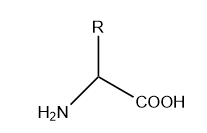
\includegraphics[width=0.3\linewidth]{aa}}%
	\subbottom[Peptide chain example]{%
		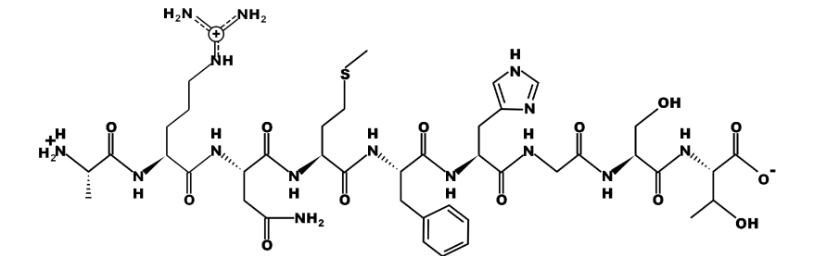
\includegraphics[width=0.6\linewidth]{aa-chain}}
	\caption{}
	\label{fig:aminoacid}
\end{figure}

\subsection{Structure}
Proteins are very complex molecules whose function is determined by its structure. In order to help understand it, we generally describe protein structure in four levels:

\begin{itemize}
 	\item Primary structure: linear amino acid sequence with peptide bonds;
 	\item Secondary structure: local folded structures, such as the $\alpha$-helix and the $\beta$-sheet;
 	\item Tertiary structure: the three-dimensional structure of the protein;
 	\item Quaternary structure: some proteins are composed by several polypeptide chains, known as subunits. The interaction between subunits gives the protein its quaternary structure.
\end{itemize}

It is worth mentioning that primary structures, i.e. sequences are more volatile since they must adapt in order for them to continue carrying on with their roles, whereas the tertiary structure is better conserved throughout these processes. This makes it so that structural conformation has an increased relevancy when it comes to analyzing proteins.

Within proteins, we can also find domains. They are considered to be independent regions in the proteins, often viewed as compact and spatially distinct units with functionalities that usually help the overall protein carry out its function. It is important to mention that similar domains can be found in proteins with different functionalities \cite{ponting2002natural}. 

\subsection{Homology}

Proteins change in order to continue carrying on their functions, which means that the ones present in organisms nowadays are the result of a long and continuous evolutionary process. Through this we can define the term homology, which in the protein context, means that two proteins share a common ancestor. Finding homology is useful because we may be able to infer unknown information of a given protein through an homologous one.

In order to determine if two proteins are homologous or not, we must analyze both their primary and tertiary structures in an attempt to find corresponding residues. Usually, we can start by checking the primary structures to see if there are identical amino acid residues in a significant number of sequential positions throughout the amino acid chain. Generally, to establish sequence homology, around $30\%$ of sequence identity must be found. If this percentage falls below this value we are required to further analyze the tertiary structures which are better preserved than sequences \cite{pearson2013introduction}. 

\section{Protein comparisons} 

As formerly mentioned, there are several uses for protein comparisons and these are made through either structural or sequential alignments. The former focuses on tertiary structures and the latter on primary structures. Despite these differences, their goals are very similar, which is to provide equivalences between residues so we can measure something that can be used to assess if two proteins are similar or not.

There are various scenarios we can come across while comparing two given proteins:
\begin{itemize}
	\item The proteins are similar in sequence and in structure: this suggests that the two proteins are homologous. Since they are similar both in sequence and structure, we can infer that they share a common ancestor and that they have the same functionalities. This scenario usually occurs when we try to group proteins with low evolutionary distances for instance. 
	
	\item The proteins are not similar both in sequence and structure: this case is most common when grouping proteins with high evolutionary distances. However, since there is nothing similar, it is hard to find any corresponding regions, which will result with the comparison between these two generate vastly different similarity measures.
		
	\item The proteins are similar in sequence but not in structure: when studying structure prediction algorithms (docking) we may face this situation, specifically when the predicted complex has a different structure from the target.
	
	\item The proteins are not similar in sequence but are in structure: once again, this case may appear when grouping proteins with higher evolutionary distances. As time passes, sequences become more prone to mutations whereas structure tends to be preserved. 
\end{itemize}

Furthermore, the use of protein comparison techniques is subject to the available information about the proteins we want to compare. We can expect two different scenarios for this work. In the first one, we have information regarding both sequence and structure, which means we can start by aligning sequences in order to find correspondences between the amino acids and only then do we proceed to the structural alignment. The second case, is when both sequences are different to the point that an alignment between them is not possible. In this case, the structural alignment is the main resource of information.

In the subsections ahead we will se how these alignments through sequence and structure work, as well as provide examples of a few algorithms.

\subsection{Sequence alignment -CITE}

To reiterate, sequence alignment is the process of arranging protein chains and looking at the present amino acids in order to identify common regions or similarities among proteins. Usually, these processes provide us with a set of matches between the amino acids from two given proteins, as can be seen in Figure \ref{fig:sequencealignment}. 

\begin{figure}[htbp]
	\centering
	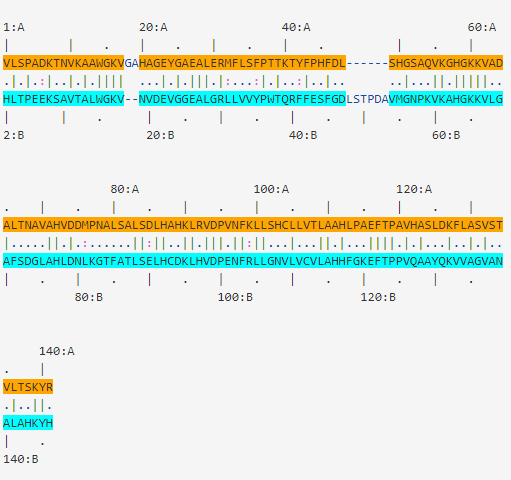
\includegraphics[width=0.4\linewidth]{sequence-alignment}
	\caption{Example of a sequence alignment between 4HHB.A and 4HHB.B -CITE-}
	\label{fig:sequencealignment}
\end{figure}

There are two types of sequence alignments: global and local. In the first type of alignment, the goal is to find the best score from alignments of entire lengths of sequences. It is most common and best used when comparing full sequences of similar lengths. The second type, local, seeks the best score from partial sequences and works best when we want to compare a shorter sequence to a larger one or a partial sequence to a whole sequence.

So far, there are a lot of algorithms and software that have been developed for sequence alignment. A few examples are FASTA \cite{lipman1985rapid}, BLAST \cite{altschul1990basic} and PSI-BLAST \cite{altschul1997gapped} for database searches, PyMol \cite{delano2002pymol} (supports commands for sequence alignments) for pairwise alignments and ClustalW \cite{chenna2003multiple} for multiple sequence alignments.

Despite the previously mentioned algorithms, let us focus on the first ones to be introduced for local and global alignment. These have served as the base for others and are still used to this day to align sequences. To describe them, let us consider two protein sequences $A = a_{1},...,a_{n}$ and $B = b_{1},...,b_{m}$. A substitution matrix $s(a_{n},b_{m})$ provides scores for comparisons between residues $a_{n}$ and $b_{m}$. These matrices can be simple ones, which attribute 1 or -1 scores in cases of matches or mismatches, or, we can use matrices that have been constructed based on statistical studies to be applied to particular scenarios. The most common ones being PAM (Point Accepted Mutation) \cite{dayhoff197822} and BLOSUM (Blocks Substitution Matrix) \cite{henikoff1992amino}. Gaps of length $k$ and $l$ are given weight $W_{k}$ and $W_{l}$, respectively. In order to find pairwise similarities, a scoring matrix $ H $ is used. 

\subsubsection{Needleman-Wunsch}

For global alignment, the Needleman-Wunsch \cite{needleman1970general} algorithm is used.

\begin{enumerate}
	\item \textbf{Initialization:} set the values of the first row and column of H according to the chosen gap penalty.
	
	\item \textbf{Matrix filling:}
		\begin{center}
			$H_{i,j} = max\begin{cases}H_{i-1,j-1} + s(a_{i},b_{j}), 
			\\  H_{i,j-1}- W,
			\\  H_{i-1,j}- W \end{cases}$
		\end{center}	
	
	\item \textbf{Traceback:} starting at the bottom right corner of the matrix, we wish to make our way into the top left corner while maximizing the score.
\end{enumerate}

\subsubsection{Smith-Waterman}

For local alignment, the Smith-Waterman \cite{smith1981identification} algorithm is used.

\begin{enumerate}
	\item \textbf{Initialization:} set the values of the first row and column of H to zero.
	
	\item \textbf{Matrix filling:} 
	
\begin{center}
	$ H_{i,j} = max\begin{cases}H_{i-1,j-1} + s(a_{i},b_{j}), 
	\\ max_{k\geq1} \left\{ H_{i-k,j}- W_{k} \right\},
	\\ max_{k\geq1} \left\{ H_{i,j-l}- W_{l} \right\},
	\\ 0\end{cases} $
\end{center}

	\item \textbf{Traceback:} starting at the highest score position of matrix H, we wish to find the path that maximizes the score and finishes in a position with value zero. 
\end{enumerate}

With this expression we cover the cases in which $ a_{i} $ and $ b_{j} $ are associated, $ a_{i} $ or $ b_{j} $ are at the end of deletions of length $ k $ or $ l $ respectively, and it also prevents the calculation of negative similarity by including a zero in such cases.

\subsection{Structure alignment} 

When comparing two given protein structures, we can usually identify three main stages. Firstly, we search both protein structures in an attempt to detect similarities among them. The second stage, consists of aligning the structures based on the found similarities. Essentially, the structure alignment process corresponds to finding the parts of one protein that best match on the other one. Lastly, the third stage is all about evaluating the alignment process, usually through some metric or score that allows us to conclude if the proteins are similar or not. The figure below \ref{fig:structurealignment} shows us an example of a structural alignment.

\begin{figure}[htbp]
	\centering
	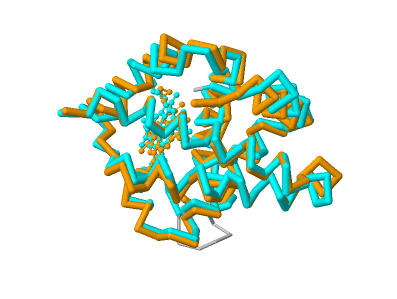
\includegraphics[width=0.4\linewidth]{structure-alignment-final}
	\caption{Example of a structure alignment between 4HHB.A and 4HHB.B -CITE-}
	\label{fig:structurealignment}
\end{figure}

%representation - optimization - alignment evaluation

To date, there are many comparison methods that use information regarding the 3-D conformation of proteins. We can split these methods in a few categories. There are approaches that break protein structures into smaller units and then analyze the relationships between these units to determine the similarity of two structures. Some examples that fit this category are: RAPIDO \cite{mosca2008alignment}, VAST \cite{gibrat1996surprising}, MASS \cite{dror2003mass}, SSM \cite{krissinel2003protein} and DALI \cite{holm1993protein}. Another possible approach that FAST \cite{zhu2005fast} and SABERTOOTH \cite{teichert2007sabertooth} explore, is obtaining a structural alignment based on pairwise residue distances. Furthermore, there are also multiple structural alignment methods such as: CBA \cite{ebert2006development}, POSA \cite{ye2005multiple}, MultiProt \cite{shatsky2004method}, MALECON \cite{ochagavia2004progressive} and MUSTANG \cite{konagurthu2006mustang}.

In the following subsections, some of the algorithms that are implemented by the available tools will be briefly described in order to provide a better idea on how they work.

\subsubsection{Superposition based on Kabsch's algorithm}

This algorithm allows us to compare two proteins by directly superimposing the structures \cite{kabsch1976solution}. It uses linear and vector algebra in order to find the best rotation and translation of two structures while minimizing RMSD. It requires a previous alignment between proteins so that we are able to measure the distance for each matched pair. An implementation of this algorithm can be found in the PyMol software \cite{delano2002pymol}.

The steps of the algorithm have a fairly complex mathematical component, which is more thoroughly explained in \cite{burkowski2008structural}, but is base steps, considering proteins P and Q, are:
\begin{enumerate}
	\item Determine the subsequences of alpha carbons to be used in the 3-D alignment:
	\begin{center}
		M(P) = $(p^{(\alpha_{1})},p^{(\alpha_{2})},...,p^{(\alpha_{N})})$
		
		M(Q) = $(q^{(\beta_{1})},q^{(\beta_{2})},...,q^{(\beta_{N})})$
	\end{center}
	\item Calculate centroids $p^{(c)}$ and $q^{(c)}$. If the atoms in the alignment do not have the same atomic weight, we can use the center of mass.
	\item Translate all the atoms to the origin of the coordinate system, so that the centroids of M(P) and M(Q) coincide. We are then working with $x^{(i)}$ and $y^{(i)}$ coordinate sets.
	\item Calculate the covariance matrix $C$, given by:
	
	$$C = \sum_{\gamma=1}^{N} y^{(\gamma)}x^{(\gamma)T}$$ 
	
	then proceed to compute its singular-value decomposition (SVD). This process allows us to express matrix $C$ as a product of matrices, $C = USV^{T}$.
	\item Compute the rotation matrix $R = UV^{T}$.
	\item Verify if $det(R) = 1$. If this determinant is negative, then we must redefine the rotation matrix to be $R = Udiag(1,1,-1)V^{T}$.
	\item Apply the rotation matrix to the $x^{(i)}$ coordinates.
\end{enumerate}

After we apply the rotation matrix to the $x^{(i)}$ coordinates we are able to determine the squared distance from each $x^{(i)}$ to its corresponding $y^{(i)}$ point. Following this, we can now perform some calculation using metrics and scores such as the RMSD.

Through this result, we can now evaluate how good the superposition is and in turn, if the two structures are similar or not.

\subsubsection{Sequential Structure Alignment Program -RESUMIR}

The SSAP \cite{orengo199636} algorithm proposes a different approach that does not require explicit superposition of the two structures. Instead, it focuses on the geometric relationships within proteins and uses them to make the necessary alignment. The concept of this algorithm is that it produces a structural alignment by constructing an alternative view for each of the protein structures, which is essentially the calculated inter-residue distance vectors between each residue. Once the vectors and their respective matrices are calculated, the algorithm calculates several new matrices that represent the differences between vectors. Then, it uses a dynamic programming approach on them to determine the optimal local alignments, which are then summed into another different matrix. Finally, by using dynamic programming again on the resulting matrix, we are given the overall alignment of the structures.

Currently, the CATH database \cite{sillitoe2014cath} provides a tool for applying the SSAP algorithm to protein data.

A more detailed version of the SSAP algorithm steps is described below:
\begin{enumerate}
	
	\item For the first step of the algorithm, we need to provide the spatial coordinates of the atoms belonging to the proteins to compare. Furthermore, we must also specify an equivalence set, which is composed by the atoms considered for the alignment. Usually, the alpha carbons are chosen for this. The sequence of coordinates for the alpha carbon atoms in proteins P and Q is represented by:
	
	\begin{center}
		$\left\{  p^{(i)} \right\}_{i=1}^{\mid P \mid}$ \qquad $\left\{  q^{(j)} \right\}_{j=1}^{\mid Q \mid}$
	\end{center}
	
	\item In the next step we describe the structural environment, also known as views, of each residue. Views are the set of vectors from each alpha carbon atom to the alpha carbon atoms of other residues in the same protein. The formal representation of the view of atom $p^{(i)}$ is
	
	\begin{center}
		$\left\{  p^{(i,r)} \right\}_{i=1}^{\mid P \mid}$
	\end{center} 
	
	where $p^{(i,r)}$ designates the vector with origin at $p^{(i)}$ and terminus at $p^{(r)}$.
	
	\item After the views are obtained, the consensus matrix follows. Using dynamic programming, we fill the matrix with values representing the similarity of the vectorial views. 
	
	\item Lastly, we want to determine the best path to go through the consensus matrix. The result of this process is an alignment that provides us with an equivalence set for the various segments of P and Q that are presumed to have structural similarity.
\end{enumerate}

\subsubsection{TM-Align}

One of the most standard algorithms for these types of alignments is TM-Align \cite{zhang2005tm}. Most times it is applied to alpha-Carbons but the algorithms' steps may be extended to other atoms of the structures. This algorithm uses an iterative heuristic process to optimize the end result. It has a complex mathematical component that it is best explained in the original paper, but a brief explanation of its main steps is provided below. 

We start off by obtaining 3 different types of alignments:

\begin{enumerate}
	\item Alignment of the secondary structures using dynamic programming in the score matrix which contains 1 or 0 values depending if the paired elements are identical or not, respectively. Furthermore, the classification of the secondary structures for a given pair of residues is assigned at this stage, taking into consideration the 5 neighboring residues. The final assignment for its secondary structure is then obtained by merging and removing isolated states.
	
	\item The second type of initial alignment consists of a gapless matching two structures. In order to facilitate this, the smaller of the two structures is aligned against the larger one and the selected alignment is the one that generate the lowest TM-score (described in the next section).
	
	\item The final type is obtained by also using dynamic programming, but this time it uses a gap penalty of -1 and the score matrix is the secondary structure score matrix combined with the distance score matrix selected in the previous type of alignment.
\end{enumerate}

Having obtained these different alignments, they are now submitted to an heuristic iterative algorithm that finds the best alignment for the two structures. This procedure begins by rotating the structures in accordance with the rotation matrices obtained in the initial alignments and this process is repeated until the alignment becomes stable.

\subsubsection{MAMMOTH}

Matching molecular models obtained from theory (MAMMOTH) \cite{ortiz2002mammoth} is another algorithm available to compute structural alignments and is the one implemented in the MaxCluster software which was used for this work and will be described in the sections ahead.

Once again, the algorithm has a heavy mathematical component and its steps are better described in the original article, but a brief description is provided below. Much like other structure alignment algorithms, MAMMOTH uses an heuristic approach in order to reduce its complexity, that is split into 4 steps:

\begin{enumerate}
	\item Start by computing the unit vectors root mean square (URMS) in the direction from $C_{\alpha}$ to $C_{\alpha+1}$ for each backbone chain and then shift the resulting vectors to the origin. Following this, it is now possible to calculate the URMS distance between the two protein segments by computing the rotation matrix that minimizes the sum of square distance between corresponding unit vectors.
	\item Use the obtained matrix in the previous step to find an alignment that maximizes the local similarity of between the structures. For this task, there is the need to calculate a similarity score, which in this case is the expected minimum URMS distance between two random sets of unit vectors. Through several of these calculations it is now possible to fill a similarity matrix S, to which dynamic programming is applied in order to build a local alignment.
	\item Next, we find the maximum subset of similar local structures whose distance falls under a given cutoff.
	\item Finally, calculate the probability of obtaining the given proportion of aligned residues.	
\end{enumerate}

\subsubsection{CE -variaveis -resumir}
One other method of obtaining a structural alignment is using \gls{CE} of an alignment path defined by \gls{AFP}. In this algorithm we define an AFP as two continuous segments (one from each structure) of the same size, aligned against each other. In short, the algorithm breaks the structures into AFP, then it builds an alignment path by adding AFP until there are none left, or the remaining ones do not satisfy a set of requirements.

Currently, there is an available web server called jCE, provided by the \gls{PDB} \cite{berman2000protein}, which is able to provide us with structural alignments using the CE algorithm.

Below, there is a more detailed explanation of the original algorithm described in \cite{shindyalov1998protein}.

Given two proteins $A$ and $B$ of length $n^A$ and $n^B$, we define the alignment path by the longest continuous path $P$ of AFP of size $m$ in a similarity matrix $S$, which represents all the possible AFP that conform to the criteria for structure similarity.

The algorithm has three main steps:
\begin{enumerate}
	\item Select an initial AFP
	\item Extend the alignment path by adding AFP in accordance with a set of restrictions
	\item Repeat the second step until we have gone through the length of each protein or until there are no more good AFP.
\end{enumerate}

Furthermore, when extending the path we must take into consideration that for every two consecutive AFP $i$ and $i+1$ in the alignment path, at least one of the following conditions must hold: there may be some gaps inserted in A or B, but not in both.

The decision of whether or not to extend the alignment path is decided according the following criteria:
\begin{enumerate}
	\item single AFP: $D_{nn} < D_0$
	\item AFP against the path: $\frac{1}{n-1}\sum_{i=0}^{n-1} < D_1$
	\item whole path: $\frac{1}{n^2}\sum_{i=0}^{n}\sum_{j=0}^{n}D_{ij} < D_1$
\end{enumerate}

Where $D_0$ and $D_1$ represent specified cut-off distances.

Given this, we must also use an heuristic to measure AFP distances and the following can be used:
\begin{enumerate}
	\item Distance calculated using an independent set of inter-residue distances, where each of them participates only once in the selected distance set.
	
	\item Distance calculated using a full set of inter-residue distances, where all possible distances except those for neighboring residues are evaluated:
	
	\item Choose the one that generates the superposition with the lowest RMSD.
\end{enumerate}

By following the steps we end up with a path built with AFP which can then be used to evaluate the structural similarity between the structures.

\subsubsection{Elastic Shape Analysis}
Another different and unique approach is ESA \cite{liu2011mathematical} which is one of the most recent approaches to compare protein structures. The main difference when compared to other approaches is that ESA considers protein backbones as continuous 3-D curves. Thus, the alignment of two structures corresponds to the alignment of the two curves representative of their backbones. These curves, known in this framework as the Square Root Velocity Functions (SRVF), are able to bend and stretch during the alignment in order for them to account for the variations between structures.

In this framework we consider a shape to be a similarity class of a curve in a Riemannian manifold. In order to obtain this similarity we require a distance metric between shapes, more specifically the geodesic path (length minimizing path), which corresponds to a curve's evolution with respect to a manifold geometry.

In short, the main idea of this approach is that we represent the protein backbones in a Riemannian manifold through SRVF functions and then find shortest path (curve evolution) from one curve to the other, with respect to the manifold's geometry.

Recently, an algorithm was developed based on this framework. The mathematical component of this algorithm is very complex and thus, better explained in \cite{srivastava2016efficient}. A summarized version of the algorithms' steps is provided below:
\begin{enumerate}
	\item Start by extracting the 3-D coordinates of the backbone to derive the initial input curve denoted by $P_{(3+k)\times n_j}^{(j)}$ for each protein $j$ of length $n_j$. The superscript $j = 1$ and $j = 2$ identifies protein 1 and 2 respectively. The superscript $(3+k)$ refers to the first x,y,z coordinates of atoms and $k$ coordinates are supplementary auxiliary information.
	
	\item Translate and scale by transforming the curves to their SRVF, represented by $Q_{(3+k)\times n_j}^{
		(j)}$.
	
	\item Recompute the SRVF $Q_1^{(1)}$ and $Q_1^{(2)}$ corresponding to a new T (piecewise linear function) for each dimension $(3+k) \times n$.
	
	\item Obtain the optimal rotation matrix through Singular Value Decomposition.
	
	\item Achieve optimal matching by using dynamic programming.
	
	\item Calculate the geodesic distance between the curves.
\end{enumerate}

As far as performance is concerned, ESA based algorithms seem to perform better than others. Despite seeming too complex mathematical wise, these approaches greatly reduce computation time, however, no known implementation was found despite this being the most promising algorithm.

\section{Measuring similarities}

In order to evaluate how good a given comparison between two structures is, we require some metric or score that we can use to assess this. Below, we can find more detailed descriptions of instances of these scores.

\subsection{Root Mean Square Deviation}

RMSD is one of the simplest ways to evaluate the similarity of a comparison of structures. It is calculated by:

$$RMSD = \sqrt{\frac{1}{n} \sum_{i=1}^{n} d_i^2}$$

where the average is calculated over the $n$ pairs of matched atoms and $d_i$ is the distance between the atoms in the i-th pair. This calculation can be applied for any subset of atoms, such as the most common $\alpha$-Carbons of whole proteins or specific subsets. 

Generally, we can interpret the result as:
\begin{itemize}
	\item If the value is zero, or close to zero \AA, it means the proteins are identical;
	\item If it ranges from 1\AA\quad to 3\AA , they are very similar;
	\item Finally, if it is greater than 3\AA, we consider that the proteins have little to no similarity.
\end{itemize}

The main issues of RMSD come from its inability to account for the variation of atom positions and sequence lengths. When these situations arise they may inflate the RMSD value for a comparison and thus, lead us to withdraw misleading conclusions. Besides this, RMSD significance may vary with protein length which means that the best alignment for two given proteins may not be the one that generates the lowest RMSD. 

\medskip
\subsection{Global Distance Test - Total Score}

An alternative to using RMSD, is the more efficient \gls{GDT-TS} \cite{zemla2003lga}. This is a procedure that also serves as a way to evaluate protein structure alignments and it is mostly used in cases where the two proteins have a very similar amino acid sequence and different structure. With this algorithm, we obtain the number of $\alpha$-Carbon pairs whose distances do not exceed the given threshold. 

Starting with an initial set of paired atoms between two structures, the GDT-TS procedure is as follows:
\begin{enumerate}
	\item Calculate a superposition for the set of atoms.
	\item Identify pairs whose distances exceed a given distance cutoff.
	\item Calculate a new superposition without the identified pairs.
	\item Repeat steps 2 and 3 until the set of atoms remains the same for two consecutive iterations.
\end{enumerate}

Usually, the GDT-TS score for two structures is calculated as an average of calculations with different distance cutoffs \cite{poleksic2009algorithms}. For instance:

$$ GDT-TS = \frac{ max C_{1\AA} + max C_{2\AA} + max C_{4\AA} + max C_{8\AA} } {4} $$
	
where the $max C_{x\AA}$ notation designates the maximum number of atom pairs under a distance cutoff of $x$ \AA. When computing a GDT score between two unrelated structures, we can usually expect a similarity value ranging from 10\AA to 20\AA, whereas the values for related structures are much higher. \cite{herbert2008maxcluster}

\medskip
\subsection{Global Distance Test - High Accuracy}

As the name indicates, the GDT-HA is very similar to the GDT-TS, however the first one uses lower RMSD cutoffs in order to be more restrictive on what it considers to be two similar structures and to give a larger impact to local matches among them. It is given by:

$$ GDT-HA = \frac{ max C_{0.5\AA} + max C_{1\AA} + max C_{2\AA} + max C_{4\AA} } {4} $$

\subsection{Template Modeling Score}

Another measure of similarity between two protein structures is the TM-score \cite{zhang2004scoring}. It was designed in order to handle two recurring problems of these kinds of metrics: the high sensibility to local variations by other metrics and the difficulty of interpreting the magnitude of the results. It solves these by taking into account the number of matching residues in both proteins and by scaling the result in order for it to range from 0 to 1, respectively. We calculate the TM-score by:

$$TM-score = \frac{1}{L} \left[ \sum_{i=1}^{L_{ali}} \frac{1}{1 + \frac{d_i^2}{d_0^2}}\right]$$

where $L$ is the length of the protein we are comparing, and $L_{ali}$ is the number of the equivalent residues in the two proteins. $d_i$ is the distance of the $i$-th pair of the equivalent residues between two structures and $d_0$ is given by:

$$d_0 = \sqrt[3]{L-15}-1.8$$

\subsection{Contact Area Difference -DEF CONTACTO-}

This similarity measure is exclusive to the study of protein-protein interactions and it represents structure similarity based on the distance of corresponding contact areas in the two structures.

Firstly, CAD applies Voronoi tessellations to each atom of both structures in order to determine the contact regions and then it determines that two atoms are in contact if they are neighbors in the resulting tessellations. After this, it represents structural similarity through:

$$CAD-score = 1 - \frac{\sum_{(i,j) \in G}^{} min \left ( \mid T_{(i,j)} -M_{(i,j)} \mid , T_{(i,j)} \right) }{\sum_{(i,j) \in G} T_{(i,j)}}$$

where $(i,j)$ represents the contacts between residues $i$ and $j$, the contact area is denoted by $T_{(i,j)}$ in the target structure and by $M_{(i,j)}$ in the modeled structure. Finally, $G$ denotes the set of all residue-residue contacts in the target structure. This score ranges from 0 to 1 with the latter symbolizing a perfect match.

\subsection{MaxSub}

Short for \gls{MaxSub}, this measure is a variation of the TM-score. The only difference between them is in the $d_0$ variable, which is set to:

$$d_0 = 3.5\AA$$ 

Since these share a great deal of similarity, they both tackle the same issues, however they produce different results. 

\section{Machine learning}
Machine learning \cite{tommitchell} \cite{ethemalpaydin2010} is a field of artificial intelligence, which can be applied to a wide range of problems, including speech, image and pattern recognition for instance. Machine learning aims to program our computers in a way that allows them to be able to learn with experience, either gained previous to, or during runtime and use it to automatically improve performance. Due to the vast application range, there isn't a particular solution that can be used to solve any problem we come across. There are two major categories in machine learning, each one best suited for a particular kind of task, they are supervised and unsupervised learning.

Supervised learning is used when we have labeled data and we want to sort or classify each entry in our dataset. Furthermore, it can even be used to make predictions for new entries in our dataset. It is called supervised because there is available labeled data that can be analyzed in order to improve our results. In other words, we can say the program is learning from past experience and using it to achieve better results when applied to new data.

Unsupervised learning is used in the opposite case, in which there is no labeled data to analyze. So instead of learning from previous experience, it focuses on analyzing the dataset and providing a better understanding and insight into our data in an attempt to find patterns, regularities, outliers and correlations among our input data.

For this work, we are trying to find similarities among proteins through their structures, however the available datasets may not include information regarding this subject, therefore we are working with unlabeled data and consequently, unsupervised learning.

\medskip
\subsection{Clustering algorithms}

Clustering is a form of unsupervised learning which aims to group elements in different clusters. Each cluster is defined by a set of elements which maximize a given similarity measure among members of the same cluster, while minimizing that same measure relative to members of other clusters.

Regarding cluster membership, it can be one of three types: exclusive, overlapping or fuzzy. Exclusive clustering dictates that each data point must belong to a single cluster. Overlapping clustering allows points to be part of more than one cluster. Lastly, in fuzzy clustering every point is a member of every cluster and that membership has a value that ranges from 0 to 1. 

The clustering process may also be complete, which requires that every data point must belong to a cluster, or partial, which allows data points not to be assigned to any cluster.

One particularly important feature of these algorithms is the ability to detect outliers, also known as noise, in our dataset. This will be useful for instance when clustering structure prediction models, in which there may be several predicted structures that can be discarded due to their greater lack of similarity.

Furthermore, clustering algorithms may belong to different categories, each of which affects how the data is processed and grouped. This causes different algorithms to produce different clusters for the same dataset. So, in order to choose an algorithm, we must first consider the kind of data we want to be processed, what kind of clusters we can expect from it and both the advantages and disadvantages of the algorithms. In the subsections ahead, some insight on the clustering categories will be provided, as well as some instances of their algorithms.

\medskip
\subsubsection{Partitional clustering}

This is one of the most popular and basic techniques for data clustering. In partitional clustering, the dataset is processed with the usual goal of maximizing a measure of similarity for members of the same clusters. During runtime, while the dataset is being clustered, the algorithms often reallocate data points to different clusters until convergence is reached. The result of these algorithms is a division of the data points into different non-overlapping clusters.

This type of clustering may be useful when predicting a protein's function, since it groups structures into non-overlapping clusters, we can expect that the protein whose function we want to predict is inserted in a group composed by those with similar structure and thus, function.

\textbf{K-means} \cite{ethemalpaydin2010} is an example of this category of algorithms. It consists of dividing the available data in \textit{k} clusters, with \textit{k} being specified by the user before the algorithm's execution. Each of these clusters is represented by the mean vector of the members of the cluster, which is the prototype of that cluster. In prototype based clustering, we assign each example to the closest prototype. The algorithm goes as follows:

\begin{enumerate}
	\item We start with an initial set of \textit{k} prototypes.
	\item Update the clusters by assigning the closest members to them.
	\item Calculate the mean vectors for each cluster with the new members.
	\item Repeat steps 2 and 3 until some stopping criteria is reached or until the updates no longer change the clusters.
\end{enumerate}

To determine the initial set of prototypes there are a few applicable methods, such as the Random Partition and Forgy methods. In the first case, each data point is assigned to a random cluster and from this attribution we calculate the initial centroid of each cluster. The second method chooses \textit{k} random examples to be centroids of the clusters.

\textit{k}-Means has a disadvantage when compared to other algorithms, which is the need to specify the $k$ number of clusters before execution. This value needs to be chosen according to the problem at hand and the available data. If it is too high or too small, the obtained clusters may contain irrelevant information.

\medskip
\textbf{Affinity propagation}

In an attempt to solve the inconveniences of having to specify the number of clusters before runtime, the Affinity Propagation \cite{frey2007clustering} algorithm was introduced. It solves this problem by introducing a message passing concept between the data points. There are two kinds of messages: availability and responsibility. 

Responsibility messages are passed between data points and based on each of their perspectives, indicate how suitable is it for others to become prototypes.  

Availability messages on the other hand, are sent by prototype candidates to all other data points and indicate how adequate the candidate seems to be based on the support it has for being a prototype.

For this algorithm, we need three components:
\begin{itemize}
	\item A similarity matrix $s_{i,k}$, filled with coefficients which indicate how alike two elements are. In this matrix,  $s_{k,k}$ indicates the tendency that an elements has to become a prototype. 
	\item A responsibility matrix $r_{i,k}$.
	\item An availability matrix $a_{i,k}$.
\end{itemize}  

In the first step of the algorithm, we initialize the availability with zeros, $a(i,k) = 0$. Next up, responsibility is calculated using:

\begin{center}
	$r_{i,k}\leftarrow s_{i,k} -\underset{k'\neq k}{max}(a_{i,k'} + s_{i,k'})$
\end{center}

Since in the first iteration, availabilities are set to zero, this matrix simply represents similarity between i and k. To update the availabilities, the following equations are used: 

\begin{center}
	$a_{i,k(i\neq k)}\leftarrow min\left ( 0, r_{k,k} + \sum\limits_{i'\notin \{ i,k \} }^{} max(0,r_{i',k})  \right)$	
	
	$a_{k,k} \leftarrow \sum\limits_{i'\neq k}^{ } max(0, r_{i',k})$
\end{center}

In order to identify the element which best represent the clusters, at each iteration we calculate for each element \textit{i}, the element \textit{k'} which maximizes the sum between the responsibility and availability. If $k' = i$, that means \textit{i} is a prototype of a cluster, otherwise, \textit{i} belongs to the cluster whose prototype is \textit{k'}.

The algorithm can stop after a fixed number of iterations, after local decisions remains constant during a few iterations, or if the exchanged messages fall below some threshold.

\medskip
\subsubsection{Hierarchical clustering}

These algorithms build clusters by either merging smaller clusters or dividing bigger ones, these approaches are called divisive and agglomerative, respectively. Either way, their goal is the same: to provide us a hierarchical view of the dataset. In the agglomerative method, each entry of the dataset forms its own cluster and at each iteration, the two most similar clusters are linked. This process is repeated until all the dataset is linked. If we are using the divisive method, instead we start with a cluster that contains all the dataset and we divide it until we have single element clusters \cite{jain1999data}. The result of either agglomerative or divisive clustering tends to be a dendrogram or a tree shaped view that displays the data hierarchy. 

This is useful for this work since it will provide us the required views and information to make an evolutionary study of proteins or to find the closest protein structure when trying to infer protein functionality.

At each iteration of an agglomerative algorithm, which is the one used for this work, we need to select the two closest groups to be merged, using some distance measure. A few examples of possible criteria are:

\begin{itemize}
	\item \textbf{Single-linkage}: join the clusters that have the shortest distance between a pair of their members.
	\item \textbf{Complete linkage}: join the clusters that have the longest distance between a pair of their members.
	\item \textbf{Ward linkage}: join the clusters that minimize the sum of squared errors, meaning the ones that incur in a smaller merging penalization.
\end{itemize}

%\textbf{Bisecting \textit{k}-Means} is an algorithm that fits this category, more specifically, the divisive approach. It uses a combination of the $k$-means algorithm and hierarchical clustering. We begin this algorithm by choosing a cluster to split. Next up is the bisecting step, on which we find two sub-clusters using the $k$-Means algorithm with $k=2$. The bisecting step is repeated for a number of iterations and takes the split that produces clusters with the highest overall similarity. This whole process is repeat until we reach the desired number of clusters.

\subsubsection{Fuzzy clustering}
Usually, clustering algorithms create partitions of our data on which each data point belong to one and only one cluster. Instead of this, fuzzy clustering \cite{jain1999data} assigns to each data point a degree of membership to every cluster.

In this work, fuzzy clustering may provide insightful information and different groupings of predicted complexes. Since generated predictions may vary in atom position or probe orientation for example, it may advantageous that complexes belong to more than one cluster.

\textbf{Fuzzy C-Means} is an example of this type of algorithms. It is based on the minimization of a criterion function, for instance:

$$J_m = \sum_{i=1}^{N}\sum_{j=1}^{C} u_{ij}^m \parallel x_i - c_j \parallel^2 $$

where $m$ is the fuzzyness coefficient and is strictly greater than 1, $u_{ij}$ is the degree of membership of data point $x_i$ to cluster center $c_j$.

Membership $u_{ij}$ and cluster centers $c_j$ are given by:

$$u_{ij} = \frac{1}{\sum_{k=1}^{C} \left( \frac{\parallel x_i - c_j \parallel}{\parallel x_i - c_k \parallel} \right) }$$


$$c_j = \frac{\sum_{i=1}^{N} u_{ij}^m * x_i}{\sum_{i=1}^{N}u_{ij}^m}$$

Considering $k$ to be the iteration steps, the algorithm goes as follows:
\begin{enumerate}
	\item Initialize the membership matrix, $u_{ij}$;
	\item Calculate the center vectors, $c_j$;  
	\item Update $u_{ij}$ for $k$ and $k+1$ iterations, with respect to $c_j$ values;
	\item Check if the difference between $u_{ij}$ for $k$ and $k+1$ iterations falls bellow a given threshold. If it does the algorithm stops, otherwise it returns to the second step. 
\end{enumerate}

\subsubsection{Density-based clustering}

In these approaches, clusters are formed based on higher density zones of the dataset. Other more scattered elements from our data may be considered noise. 

For this work, density-based clustering may aid in the detection of noise in protein docking complexes and as such, remove structures that do not resemble the target complexes.

\textbf{DBSCAN}: as described previously, there are a few issues with prototype-based clustering algorithms: determining the number of clusters and the inability to consider relationships among points. 

The \gls{DBSCAN} \cite{ester1996density} algorithm introduces a different approach which deals with these problems. Through a set of definitions applied during execution, the algorithm can filter out noise, establish relations among data points and form clusters accordingly.

\begin{itemize}
	\item \textbf{Definition 1}: The Eps-neighborhood of a point p, denoted by $N_{Eps}(p)$ is defined by $N_{Eps}(p) = \left\{q\in D\mid dist(p,q)\leq Eps\right\}$.
	
	\item \textbf{Definition 2}: (directly density-reachable) A point p is directly density-reachable from a point q with respect to Eps, MinPts if:
	
	\begin{enumerate}
		\item $p \in N_{Eps}(p)$ and
		\item $\mid N_{Eps}(p) \geq MinPts \mid$ (core point condition)
	\end{enumerate}
	
	\item \textbf{Definition 3}: (density-reachable) A point p is density-reachable from a point q with respect to Eps and MinPts if there is a chain of points $p_{1},...,p_{n}, p_{1} = q,p_{n}=p$ such that $p_{i+1}$ is directly density-reachable from $p_{i}$.
	
	\item \textbf{Definition 4}: (density-connected) A point p is density-connected to a point with respect to Eps and MinPts if there is a point o such that both, p and q are density-reachable from o with respect to Eps and MinPts.
	
	\item \textbf{Definition 5}: (cluster) Let D be a database of points. A cluster C with respect to Eps and MinPts is a non-empty subset of D satisfying the following conditions:
	
	\begin{enumerate}
		\item $\forall p,q$ if $p \in C$ and q is density-reachable from with respect to Eps and MinPts, then $q \in C$. (Maximality)
		\item $\forall p,q \in C$: p is density-connected to q with respect to Eps and MinPts. (Connectivity)
	\end{enumerate}	
	
	\item \textbf{Definition 6}: (noise) Let $C_{1},...,C_{k}$ be the clusters of the databases D with respect to parameters $Eps_{i}$ and $MinPts_{i}$, i = 1,...,k. Then we define the noise as the set of points in the database D not belonging to any cluster $C_{i}$, i.e. noise = ${p \in D \mid \forall i: p \notin C_{i}}$.
\end{itemize}

The algorithm starts by receiving the entire set of points as input and then it chooses an random point that has not been visited yet. Afterwards, it fetches the neighborhood of this point to be compared against MinPts. If the size of its neighborhood is lower than MinPts, this point is labeled as noise, otherwise it is a core point and it forms a cluster to which it joins its neighborhood. If there is a neighbor of this point which is also a core point, the two clusters are merged. This process is repeated until all points are visited. It is worth noting that a point which was labeled as noise in a given iteration can become part of a cluster in further iterations.

The authors of the article mention an heuristic to determine the values for parameters MinPts and Eps. These values are set to those of the least dense cluster in the data set. Since they represent the lowest density that is not considered to be noise, it is effective to use them as global parameters.

This algorithm does in fact solve the issues of prototype-based clustering, however it has its own flaws, as it is not very effective when the clusters have varying densities and the dataset has high dimensionality.

\subsubsection{Shared Nearest Neighbors}

As we have established, there are some challenges that arise when using clustering algorithms: \textit{k}-Means does not do well with clusters of different sizes or non-globular shapes, DBSCAN fails when the dataset has varying densities or high dimensionality, etc.

The \gls{SNN} algorithm is another approach that addresses a lot of these issues. It uses the Jarvis-Patrick \cite{jarvis1973clustering} approach to define the similarity between a given pair of points, which takes into account how many nearest neighbors they have in common. This definition removes the problems with varying densities. Furthermore, the algorithm identifies and builds clusters around core points. These clusters also deal with noise, by grouping only data from regions of uniform density. One other feature of this algorithm, is that it finds clusters that other approaches overlook, such as those in lower density regions and also single element clusters.

This algorithm can be used in functionality prediction through its concept of neighborhood, since we may clearly identify other structures that are most similar to the one whose function is unknown. It may also be used in protein docking in order to group the predicted complexes that are most similar to the target.

Since one of the cores of SNN belongs to the Jarvis-Patrick algorithm, a brief description of it is provided below:

\begin{enumerate}
	\item Start by calculating the set of $k$ nearest neighbors for each data point.
	\item Then, merge points to form clusters if they share at least $K_{min}$ of their nearest neighbors.
\end{enumerate}

To determine the nearest neighbors, a distance cutoff is required, such as the RMSD of two structures.

As stated in \cite{ertoz2003finding}, the SNN algorithm goes as follows:
\begin{enumerate}
	\item \textbf{Compute the similarity matrix.} (This corresponds	to a similarity graph with data points for nodes and edges whose weights are the similarities between data points.)
	\item \textbf{Sparsify the similarity matrix by keeping the \textit{k} most similar neighbors.} (This corresponds to only keeping the k strongest links	of the similarity graph.)
	\item \textbf{Construct the shared nearest neighbor graph from the sparsified similarity matrix.} At this point, we could apply a similarity threshold and find the connected components to obtain the clusters (Jarvis-Patrick algorithm.) 
	\item \textbf{Find the SNN density of each point.} Using a user specified parameters, Eps, find the number points that have an SNN similarity of Eps or greater to each point. This is the SNN density of the point. 
	\item \textbf{Find the core points.} Using a user specified parameter, MinPts, find the core points, i.e., all points that have an SNN density greater than MinPts.
	\item \textbf{Form clusters from the core points.} If two core points are within a radius, Eps, of each other, then they are placed in the same cluster.
	\item \textbf{Discard all noise points.} All non-core points that are not within a radius of Eps of a core point are discarded.
	\item \textbf{Assign all non-noise, non-core points to clusters.} We can do this by assigning such points to the nearest core point. 
\end{enumerate}

It worth mentioning that this process also uses what is essentially the DBSCAN algorithm, in steps 4 through to 8. Thus, the parameters MinPts and Eps are determined according to the non-noise least dense cluster. 

In regards to proteins, we can use this technique to find the nearest neighbors of a given protein, which correspond the ones that are most similar to it. 

\subsection{Cluster evaluation}
Several authors have studied and applied cluster techniques, however, when it comes to what a good cluster looks like, it seems that they do not reach a consensus. Since clustering can be applied to a vast range of problems, good clusters vary with the problem at hand. 

Despite this, some evaluation criteria have been developed and usually fit one of two categories, internal and external \cite{duda2012pattern} \cite{rokach2005clustering}.

\subsubsection{Internal quality criteria}

These types of metrics focus on evaluating the compactness of the clusters, which in other words is equivalent to measuring the homogeneity of members of the same cluster. In this case, it will allow us to see if the proteins that belong to the same clusters are similar to one another.

\medskip
\begin{itemize}
\item \textbf{Calinski-Harabasz score:} this score represents the ratio between the within cluster dispersion and the between cluster dispersion. This score is given by the following equations:

$$CH(k) =\left[ \frac{B(k)}{W(k)}\right] \times \left[\frac{\left(n-k\right)}{\left(k-1\right)}\right]$$

Where $N$ is the number of data points, $k$ corresponds to the number of clusters and $W_k$ and $B_k$ represent the within cluster and between cluster dispersions, respectively, which in turn are obtained by:

$$W_k = \sum_{q=1}^k\sum_{x\in C_q}(x-c_q)(x-c_q)^T$$

$$B_k = \sum_q n_q(c_q-c)(c_q-c)^T$$

Here, $C_q$ is the set of points that belong to cluster $q$, $c_q$ is its center and lastly, $n_q$ is the number of its data points. By looking at the way this score is calculated, we can conclude that it tends to be higher when the clusters are dense and well separated, thus, the higher the result the better the model used to cluster the data. \cite{calinski1974dendrite} \cite{scikitlearn}

\medskip
\item \textbf{Silhouette score}: is the overall representation of how well each data point fits its cluster. The silhouette score depends on:

\begin{itemize}
	\item $a(i)$ = average dissimilarity of $i$ to all other objects of cluster A.
	\item $d(i,C)$ = average dissimilarity of $i$ to all objects of cluster C. 
	\item $b(i)$ = $\min\limits_{C \neq A} d(i,C)$
\end{itemize}

It is possible for us to use different distance measures to determinate the dissimilarity, such as the Manhattan or Euclidean distances. To calculate the silhouette score for a given point, we use the following expression:

$$s(i) = \frac{b(i)-a(i)}{\max\{a(i),b(i)\}}$$

From this definition, we can infer that the score for a data point will range from -1 to 1. \cite{rousseeuw1987silhouettes} \cite{scikitlearn}

\end{itemize}

\subsubsection{External quality criteria}
These measures are more useful when the overall structure of the clusters can be compared to some predefined classification of the data \cite{rokach2005clustering}. In this work, the datasets that contain the data to be clustered, already have groups and hierarchies formed within them. SCOP and CATH are databases with hierarchies aimed at better understanding evolutionary relationships, hence have their own classification for the structures and can be used to compare the ones obtained with the clustering algorithms. Similarly, the Uniprot database has information regarding domain functionality, which can be used to check if the proteins in our clusters share the same functionality as the protein whose function we are attempting to predict. 

The external criteria mentioned ahead will aid us in performing these comparisons and in turn assess the performance of the clustering algorithms in order to determine if they are generating good or bad results:

\begin{itemize}

\medskip
\item \textbf{\gls{ARI}}: \cite{scikitlearn} \cite{hubert1985comparing} represents the consensus between the ground truth $C$ and the labels attributed by the clustering algorithm $K$. Considering $a$ as the number of pairs that belong to the same clusters in $C$ and in $K$, and $b$ as the number of pairs in different clusters, we have:

$$RI = \frac{a+b}{C_{2}^{n_{samples}}}$$

$$ARI = \frac{RI - E\left[RI\right]}{max(RI)-E\left[RI\right]}$$

where $C_{2}^{n_{samples}}$ represents the total number of possible pairs among the data and $E\left[RI\right]$, the expected Rand Index of random labellings.

The closer to 1 this score is, the more the cluster labels resemble the ground truth, if it is 0 or negative the worse it is.

\medskip
\item \textbf{Adjusted Mutual Information}: Similar to the previous metric, AMI also returns 1 if the two provided input clusterings are in complete accordance with each other and 0 or a negative value if its the complete opposite situation. The difference is that AMI accounts for chance and is biased towards clusterings with a higher amount of clusters.

$$ARI(U,V) = \frac{MI(U,V)-E\left\{ MI(U,V) \right\}}{max \left\{ H(U),H(V) \right\} - E\left\{ MI(U,V) \right\}}$$

MI can be thought of as a measure reduction in uncertainty for predicting outcome of a system after we have observed the other part, which in this case is the existing classification of the data. A more detailed description can be found in its original paper. \cite{vinh2010information} \cite{scikitlearn}

\medskip
\item \textbf{Homogeneity}: 
 
This measure reflects the degree to which data points are similar to each other. In other words, a clustering result satisfies the homogeneity criteria if the members of each cluster belong to a single class \cite{rosenberg2007v} \cite{scikitlearn}. It is given by:

$$h = 1 - \frac{H(C|K)}{H(C)}$$

Where $H(C|K)$ is the conditional entropy of the classes depending on the cluster assignments and $H(C)$ the entropy of the classes. These coefficients can be determined through:
 
$$H(C|K) = - \sum_{c=1}^{|C|} \sum_{k=1}^{|K|} \frac{n_{c,k}}{n} \times \log \left( \frac{n_{c,k}}{n_k} \right)$$
 
$$H(C) = - \sum_{c=1}^{|C|} \frac{n_c}{n} \times \left( \frac{n_{c}}{n} \right)$$
 

\medskip 
\item \textbf{Completeness}:
 
Since homogeneity only focuses on assessing the quality of the data point clustering, we need a counterpart to it, in order to evaluate if all the available data points have been assigned to a cluster. This is essentially what completeness is: a measure that reflects the portion of the total data points that have correctly been assigned to a cluster. It is given by:

$$c = 1 - \frac{H(K|C)}{H(K)}$$

Both the conditional entropy and cluster entropies can be calculated in a similar fashion to that of the homogeneity measure \cite{rosenberg2007v} \cite{scikitlearn}.

\medskip
\item \textbf{V-measure}: 

Is defined as the harmonic mean between the homogeneity and completeness measures:

$$v = 2 \times \frac{h \times c}{h + c}$$

Its value ranges from 0 to 1. \cite{rosenberg2007v} \cite{scikitlearn} 

\end{itemize}
 
\chapter{Available data and tools} 

This chapter will provide a brief description of the available tools that were to developed the required code and the platforms that hold useful data for this work. 

\section{Alignment tools}

\subsection{BioPython}

\cite{cock2009biopython}

This is a library developed for the Python programming language which provides a wide range of utilities for protein data processing. It allows its users to parse PDB and SCOP files, for instance, and access more complex information regarding each protein, however, it seems this library is more oriented towards protein sequences. Nevertheless it may still be used as a tool for structural alignment and the subsequent RMSD calculation.

\subsection{BioJava}

\cite{holland2008biojava}

This is the Java library that powers the jCE tool available on the PDB. It is a complex and powerful library that is able to load protein files and calculate both sequence and structural alignments. As far as structure similarity measures are concerned, RMSD and TM-score are available. 

\subsection{Clusco}

\cite{jamroz2013clusco}

Clusco is one of the most complete tools in the context of this work. It provides an easy way for its users to calculate structure alignments and cluster proteins according to the results. It can compute RMSD, GDT, TM-score, MaxSub and CMO for a given structural alignment. Despite this, it was not chosen as the main tool since initial experiments have shown that the input for the all against all comparison cannot exceed 10 structures.

\subsection{jCE}

\cite{prlic2010pre}

Available for download or to be used online on the PDB website, the jCE tool is powered by the BioJava library and provides us with protein alignments and visualization tools. Even though each alignment generates a great deal of information, as far as structural similarity measures are concerned, only the RMSD is displayed.

\subsection{MaxCluster}

MaxCluster is a protein alignment and clustering tool. It allows us to compute RMSD, GDT, TM-score and MaxSub for a given alignment of two structures using the MAMMOTH algorithm. This program does support list processing, however it is not useful for this work since there are thousands of files to be loaded into memory simultaneously which is not feasible and thus, the single alignment feature was used. \cite{herbert2008maxcluster}

\subsection{TM-Align and TM-Score}

The creators of TM-Align algorithm and TM-score measure have also programmed two tools, which are freely available online and can be used to obtain protein alignments and structure similarity measures. Although these are both fast tools that calculate alignments, they have their drawbacks regarding this work's objective. 

The TM-score program is one that also calculates RMSD, TM-score, MaxSub, GDT-HA and GDT-TS. It was initially considered for this work, however it is not meant to be used on proteins whose sequences are very different since according to the authors, it is limited to comparing models based on their given and known residue equivalence.

TM-Align on the other hand, may be employed to align proteins with different sequences but it is also limited by the fact that it only calculates RMSD and TM-score.

\section{Languages and libraries}

\subsection{Python}

Python a is very popular, high-level and general-purpose programming language. It can be used to build standalone applications, automate tasks and many others. Besides these uses, Python has been one of the most used languages in machine learning since it provides several powerful libraries designed for the type of tasks the field requires.

\textbf{Matplotlib}

A data visualization library. Matplotlib is a common and flexible tool which allows the user to create a wide range of plots, such as 2-D histograms, bar charts, scatter plots and tables. \cite{Hunter2007}

\medskip
\textbf{Numpy}

Another one of the most popular Python libraries. Numpy provides its user with N-dimensional arrays, easy to use array manipulation and transformation as well as complex algebraic computations with overall better performance than native arrays. \cite{walt2011numpy}

\medskip
\textbf{Scikit-learn}

Clustering algorithms are one of the main aspects of this work, which is why the Scikit-learn \cite{scikitlearn} library was used. It was developed for the Python programming language and it provides us with implementations of supervised and unsupervised algorithms, among which, are clustering functions and evaluation methods.

\subsection{R}

As opposed to Python, R serves a more specific role, that of statistical computing and data visualization. It is a high-level programming language whose abstractions facilitate what in other languages would be a more complex task, such as loading data and plotting graphics.

\textbf{DBSCAN}

This is a clustering library \cite{hahsler2017dbscan} which implements a collection of popular algorithms, most of them based on the density clustering approach. The most relevant algorithms present are: \gls{DBSCAN}, HDBSCAN, OPTICS and \gls{SNN} Clustering.

\medskip
\textbf{ppclust}

Is yet another clustering library \cite{ppclust2018}, however the algorithms it implements are focused on probabilistic clustering. It features, among others, the Fuzzy C-Means algorithm.

\medskip
\textbf{Factoextra}

This a data visualization tool \cite{kassambara2016factoextra}, which provides functions that allow the user to easily extract algorithms’ summaries as well as plot said information.

\section{Protein data}

\medskip
\textbf{CAPRI}

The Critical Assessment of PRedicted Interactions (CAPRI) \cite{janin2005assessing} is an experiment designed in order to test protein docking algorithms. CAPRI is a blind experiment in the sense that the participants do not know the structure that they are trying to predict. However, after each round is finished the results are evaluated and made available to the public. Thus, the data on this platform can be used in order to cluster protein docking models according to the target information.

\medskip
\textbf{CASP}

The \gls{CASP} \cite{moult1995large} is the complement of the CAPRI experiment. After the predictions are submitted in the CAPRI experiments there is the need to evaluate and rank the models produced by the participants' algorithms, which is exactly what \gls{CASP} does. Having finished the evaluation of each experiment, several resulting files are made available to the public. These files contain very useful information for this work, specifically, the coordinates of the prediction and target models and summaries of the experiments, which save us the trouble of having perform any alignments. 

\medskip
\textbf{CATH}

The \gls{CATH} \cite{sillitoe2014cath} protein structure database is an online platform that holds data regarding evolutionary relationships of protein domains. Currently, it contains 95 million protein domains which are classified into 6119 superfamilies. The acronym originates from the hierarchical classification of the domains: 
\begin{itemize}
 	\item Class (C): ranges from 1 to 4 and describes the classification of the folds, respectively, mainly $\alpha$, mainly $\beta$, mixed $\alpha \ \beta$ and lastly, little secondary structure.
 	\item Architecture (A): describes the three-dimensional conformation of the secondary structures.
 	\item Topology (T): holds information regarding how the secondary structure elements are connected and arranged.
 	\item Homologous superfamily (H): level that indicates if there is evidence of common ancestry.
\end{itemize}

Furthermore, protein domain superfamilies were subclassified into functional families. These are groups of protein sequences and structures that have a high probability of sharing the same function, which is information that can be used to test the accuracy of the results of clustering algorithms.

\medskip
\textbf{PDB}

The \gls{PDB} \cite{berman2000protein} is the largest repository of information regarding 3-D structures of biological molecules, including proteins. It is maintained by the Research Collaboratory for Structural Bioinformatics (RCSB) and it is one of the most important resources for studying protein structure. Currently, this platform freely supplies data for researchers and other databases, which is available in \gls{PDB} format and includes information such as atomic coordinates, molecule names, primary and secondary structures. 

\medskip
\textbf{SCOP}

The \gls{SCOP} \cite{murzin1995scop} database contains the description of the relationships of all its known protein structures. It is hierarchically organized in four levels:
\begin{enumerate}
	\item Superfamily : describes information of far evolutionary distances, meaning the proteins have low sequence identity, however through structure it is possible to trace common ancestors.
	\item Family : describes information of near evolutionary distances, but in this classification sequence and structural similarities are more evident.
	\item Fold : describes geometric relationships among the proteins. Specifically, this level indicates that proteins have common folds if they have similar secondary structures.
	\item Class : describes the classification of the folds, which are: all $\alpha$-helices, all $\beta$-helices, $\alpha \beta$ for those with both, $\alpha + \beta$ for those with both and are largely segregated and finally, Multi-domain is the classification for the domains that have no current known homologues.  
\end{enumerate}

With the information contained in this database it is possible to perform an evolutionary study of proteins. By clustering their structures in order to find similar protein groups, we can then compare the obtained results with the ones present in the database. This will allow us to test both the effectiveness of the clustering algorithms and the measures used to compare protein structures.
 
\medskip
\textbf{Uniprot}

Uniprot \cite{uniprot2014uniprot} is a collection of resources regarding protein information. Its composed of three databases that collectively store the different types of information of this platform:

\begin{itemize}
	\item Uniprot knowledgebase (UniprotKB): is the central hub for the collection of functional information on proteins. Each entry contains detailed information on each protein, such as their amino acid sequence, protein name and taxonomy.
	\item Uniprot reference clusters (UniRef): contains clustered sets of protein sequences originating from UniprotKB.
	\item Uniprot archive (UniParc): stores most of the available and known protein sequences.
\end{itemize}
 
The data from UniprotKB may prove to be useful for this work when attempting to predict a protein's function based on its structure since it provides annotations for \gls{SCOP} domains.


\chapter{Approach - Recent}
%At first, the work plan seemed well detailed enough to cover most of the aspects this dissertation would require. However, it was quickly revealed that there were some issues with it, namely, the lack of availability or functionalities of some of the tools that were first mentioned which would be used to perform the alignments of the structures and their subsequent clustering. Due to these issues, the R language was used to complement Python's Scikit-Learn library in the sense that it provided implementations of the Fuzzy C-Means and Shared Nearest Neighbors Clustering algorithms. Regarding the alignments, instead of the available PDB tools, the MaxCluster program was used.
This chapter contains a detailed description of how the different tasks and goals established were accomplished

\section{Sampling}

The amount of protein structure files present in the SCOP database exceeds the hundreds of thousands, and thus it becomes an unfeasible task to obtain a complete similarity matrix with the available hardware. Given this there is the need to sample the data in a way that we can obtain a wide range of alignments in terms of their quality. We want there to be a lot of different structures in our sample because this way the amount of very similar and very different structures will be low. This is a good thing because in extreme cases of either similarity or dissimilarity, any single structure similarity measure suffices. It is the middle ground of these ranges that we want to study, since it is most likely where there will be relevant changes in the classification and also where the shortcomings of the measures will manifest themselves.

This is why the sample chosen must contain more intermediate values, since it is in these situations that the used similarity measures are most likely to misrepresent the differences between two structures and as such, it is where we will try to compensate with another measure.

With these restrictions in mind, a few samples were chosen from the SCOP hierarchy. The structures taken were chosen from specific classes and folds, for instance, $a.1.$ would return every structure from every family and superfamily that was labeled with a class $\alpha$ and fold 1. 

\section{Alignment computation}

In order to start clustering the structures, it was essential to obtain the structural alignments and the resulting values. To accomplish this task, the MaxCluster program was used. This piece of software is implemented in the C programming language which makes its runtime extremely low for single alignments. Maxcluster supports list processing that allows the computation of all against all alignments for the given input structures, which is both faster to calculate and easier to process than single alignments, however, once again, this feature is limited by hardware and as such the sample size must be restricted to a smaller amount.

Besides the structural alignments, the sequence alignments were also computed using ClustalW. Much like the previous program, there is also the possiblity of calculating single and list alignments, however, the computation of the sequence alignments is much lighter than that of the structures.

\section{Data processing} 

From the all against all alignments, Maxcluster outputs a single file that contains two types of information: the numbers that represent each structure within each Maxcluster execution, ranging from 1 to the amount of structures in input, and the pairwise similarities for each structure combination. Similarly, ClustalW also outputs the sequence identity percentage matrix, which has a different format than that of the Maxcluster files but needs to be processed all the same.

These resulting files were then processed in a way that allowed for the extraction of the mentioned matrices. This consisted of loading the data to 2D numpy arrays and symmetrizing them.

Once the symmetrical similarity matrix were obtained, the distance matrix followed. To accomplish this task, we assumed an Euclidean space which allowed us to calculate the distance between each pair of structures. From this, the distance matrix was obtained and the clustering phase began.

One issue that was raised in the early stages of the experiment was that the studied structure similarity measures are on different scales. RMSD for instance, starts from 0 and does not have a limit, while GDT is presented as a percentage, from 0 to 100. Since we aim to combine different similarity measures through their respective distance matrices, there is the need to rescale the data.

There are two main ways of achieving this, those being normalization and standardization, which are obtained by:

	 $Normalization: z_i = \frac{x_i - min(x)}{max(x)-min(x)}$

	 $Standardization: z = \frac{X - \mu}{\sigma}$

In order to choose the most appropriate way to scale our data, its density estimation was determined. Usually, when the data distributions are more uniform, normalization is the preferred approach, which was the case as we can see in the distributions shown below, in figure \ref{fig:kde}.

\begin{figure}[htbp]
	\centering
	\subbottom[RMSD distribution]{%
		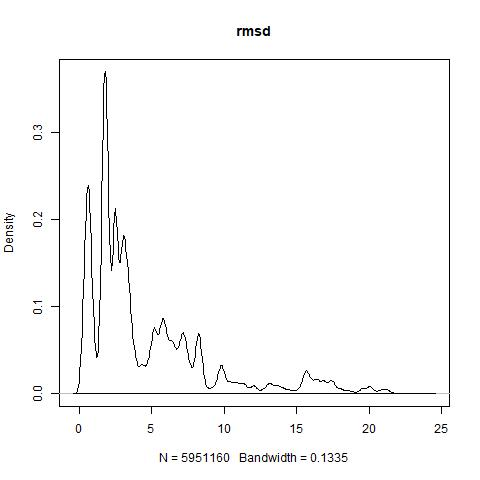
\includegraphics[width=0.3\linewidth]{rmsd}}%
	\subbottom[GDT-HA distribution]{%
		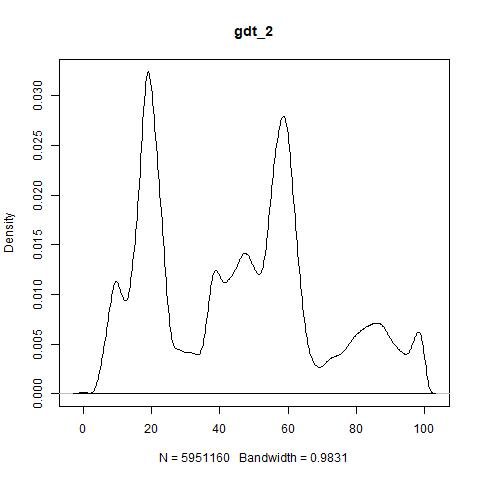
\includegraphics[width=0.3\linewidth]{gdt2}}%
	\subbottom[GDT-TS distribution]{%
		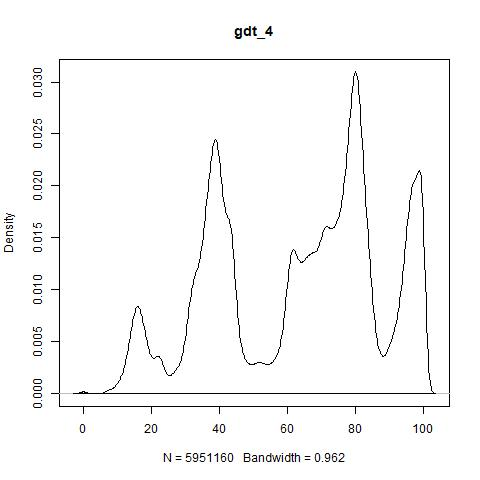
\includegraphics[width=0.3\linewidth]{gdt4}}
	\caption{}
	\label{fig:kde}
\end{figure}

After obtaining the alignment matrices, we also needed to calculate the distances between points and thus, the Euclidean distance was chosen for this. It is given by:

	$$d(p,q) = \sqrt{\sum_{i = 1}^{n}\left( p_i - q_i \right)^2}$$


\section{Clustering}
Having obtained the distance matrices, the clustering process was next. One of the algorithms that was considered was DBSCAN. Ultimately, it was not used as it was deemed too ineffective for the task at hand. This was due to the algorithm's approach to clustering, since its parameters are extremely hard to adjust to our data in the sense that it does not allow us to directly state how many clusters we wish to be formed. Besides the issue of estimating optimal parameters, the is also the issue that DBSCAN uses the density concept to cluster the data, which means that depending on its entry parameters there may be structures that are labeled as noise and as such, will not be given a label which in turn implies that the final cluster evaluation will not take into account some of the input structures, thus hindering the experiment's results

Given this, the studied algorithms were agglomerative and k-medoids. Both of these also receive distance matrices as input and one the most important aspects is that we can choose how many clusters we want the data to be split into. As opposed to DBSCAN, these algorithms also label every structure in our dataset.

The experiment itself started by clustering the distance matrices of the mentioned similarity measures: RMSD, GDT-HA and GDT-TS. These provided us with the reference values (cluster evaluation metrics) that we wished to optimize, specifically the RMSD classifications, since it is the one used in the SCOP database. 

So far, we have established that there is a need to combine different structure similarity measures. However, this is not an easy task since theoretically we can have every number within the [0,1] range as weights for the considered measures. In an effort to mitigate this issue, only weights with two decimal numbers were considered. Having gotten past this, there is now a need to find the best combination of weights among the different measures, for which a genetic algorithm was used. This is a powerful tool that can be applied in optimization problems, as is the case.

The general steps of a genetic algorithm are the following:
\begin{enumerate}
	\item Initialize population randomly
	\item Evaluate the fitness of the population
	\item Select the individuals from which the new generation will be formed
	\item Crossover
	\item Mutation
	\item Repeat steps 2-5 for N generations or until convergence
\end{enumerate}

For this particular problem, our individuals are made of three numbers, each of which corresponds to the weight that a given protein similarity measure will take during the clustering process. As for fitness, the algorithm uses the ARI clustering evaluation metric, meaning that we are trying to optimize the weights with respect to the existing SCOP classification. After determining the individual whose weights generate the best ARI, we then calculate its internal clustering metrics. This way, we are guaranteed to obtain the weights that produce results that most closely resemble the existing classifications. It should be mentioned that it is to be expected that the external metrics should be lower than the base case, since we are using other similarity measures and comparing the results with others obtained with respect to RMSD. However, the internal metrics are expected to surpass those of the base classification.

\chapter{Results}

In this chapter, the clustering results are presented along with a discussion regarding whether or not the results were as expected, if each algorithm is appropriate for this type of data and the which are the best structural similarity measures.

\section{Analysis}

As was mentioned in the previous chapter, the experiments began by obtaining the base clustering results, specifically, the metrics that originated from the different algorithms when applied to the individual distance matrices.

\begin{figure}[htbp]
	\centering
	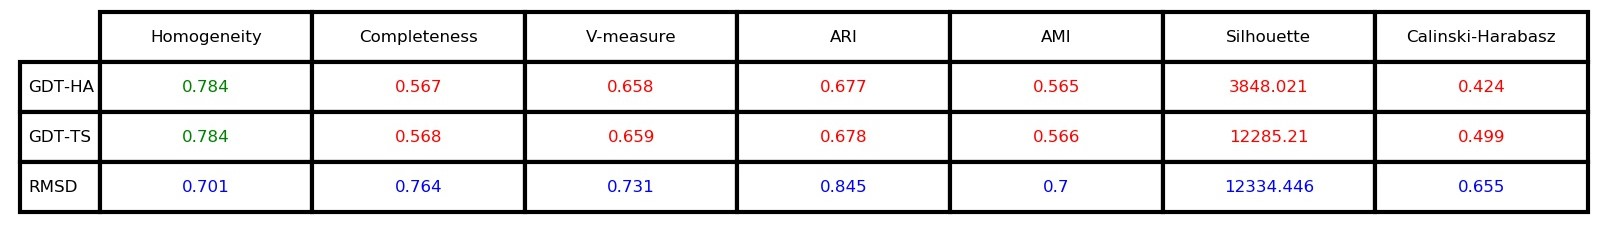
\includegraphics[width=1.1\linewidth]{average.jpeg}
	\caption{-CITE-}
	\label{}
\end{figure}

%TODO
The table displayed above shows us the results obtained when applying the hierarchical clustering algorithm with average linkage. In said table, we can see that the row that corresponds to the RMSD clustering metrics has their values in blue, this is because RMSD is the protein similarity measure by which SCOP organizes its hierarchy and as such, its values serve as a reference to which all other values in the table will be compared to. 

At this point, it was to be expected that at least the external metrics would perform worse for other similarity measures, since the base classification is obtained mainly through the RMSD alignments. On the other hand, the internal metrics for the other measures could have performed better, since they are not tied to an already existing classification. For this particular sample, $a.1$, changing the linkage type to complete changed nothing at all and thus, its corresponding table is exactly the same as the one displayed previously.

On the other hand, the k-Medoids algorithm produced some interesting results, as we can see in the table below:

\begin{figure}[htbp]
	\centering
	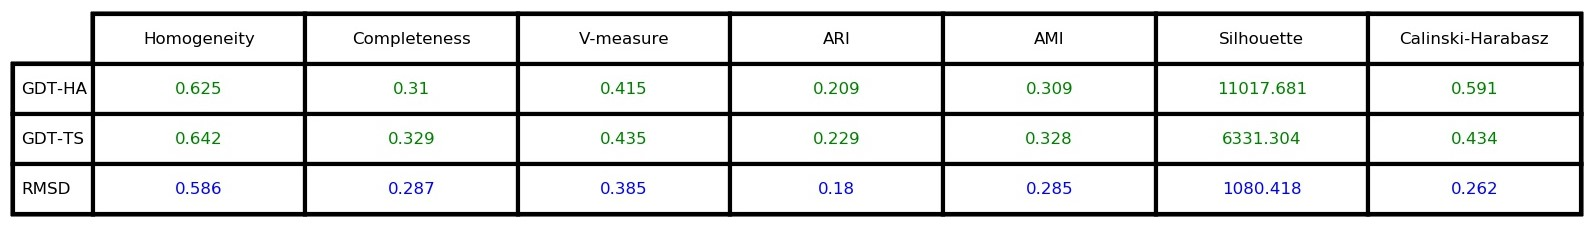
\includegraphics[width=1.1\linewidth]{medoids.jpeg}
	\caption{-CITE-}
	\label{}
\end{figure}

Although we can see that there were several improvements from the base RMSD classification, we must be careful in this analysis. In this case, we should not pay much attention to the external clustering metrics due to them being compared to the classification attributed by the SCOP hierarchy, which uses a hierarchical clustering algorithm. Given this, we should focus on the internal metrics, which are very surprising due to the disparity between them.

%CONTINUE

\section{MISC}

%SEQUENCES ARE BAD
The poor results displayed in the sequence row are also to be expected. The way that the data was sampled forces the resulting sets to contain many diverse proteins, which are classified into superfamilies. As discussed previously, proteins within the same superfamily share common ancestors, however, the traces of similarity through sequence are very scarce, which means that the amino acid chains are not well suited to used by themselves in the clustering process.

%SCOP CLUSTERING
To reiterate, the SCOP database uses a mixture of both manual and automatic methods to group the present domains into its hierarchy which use RMSD. Given this the first steps of this experience should be to determine the reference values that the other similarity measures will be compared to.

\chapter{Conclusion}

In this chapter, the results from the experiences are summarized. Furthermore, we also mention the limitations encountered and discuss future prospects regarding this work.

\section{Final remarks}

Overall, the results that were obtained are very favorable. As it turns out, by adding another dimension to the structural alignment data we can more accurately form protein groups. This holds true for the databases used since according to the clustering evaluation there was a big

It was also discovered that algorithms that allow us to customize the definition of a cluster, namely Affinity Propagation, DBSCAN and SNN are not the best suited for the task of clustering protein structures. This is due to the fact that two of these algorithms have noise detection, which is as good as it is harmful since it removes both good and bad data, and also because all of them require complex parameterization that must be optimized for each case, thus, becoming impractical despite its viability.

Summing up, the overall results were as predicted, however, the improvement was not as big as expected since it seems that the better similarity measure combinations are the ones that contain GDT-HA but it barely edges other combinations.



-overall yes-
-complementary measures improve clustering-
-resumo dos resultados-
-qual o melhor algoritmo para cada contexto-
-discutir se foram os resultados esperados-
-noise detection useless as there are very few outliers-
-future: more measures that werent tested-

\section{Detected limitations}



\section{Future work}

In future prospects, it would be interesting to see the protein databases mentioned in this document would be willing to use their resources to recompute their alignments in order to see if the current labels and cluster representatives would either change or remain the same when represented by complementing similarity measures. This of course implies that there would be no restrictions in data or sample size and therefore should show the most accurate results using the methodology that was studied during the course of this work.

Furthermore, classifications for new entries in the databases could also be experimentally obtained in order to verify if this clustering methodology for unknown label prediction may be applied in practice. 

%-usar 3 medidas-

\section{Source code}

The source code that was written to accomplish the different tasks this work required is available for consultation at \url{https://github.com/PArguelles/protein-clustering} 
